\subsection{Decoding}

Decoders \cite{cho-etal-2014-learning} form an integral part of sequence-to-sequence models in natural language processing tasks, and they are constructed as a multi-layered architecture of recurrent elements, such as Long Short-Term Memory (LSTM) units, Gated Recurrent Units (GRUs), or other analogous structures. The primary responsibility of a decoder is to generate an output sequence by predicting an output, denoted as y, for each time step. This output sequence can be a series of words, phrases, or even entire sentences, depending on the specific problem being addressed.

At each time step, the current recurrent unit within the decoder receives a hidden state from the preceding recurrent unit. This hidden state encapsulates the information gathered up to that point and serves as a vital input for the current recurrent unit to make an informed prediction. Moreover, decoders can also incorporate attention mechanisms to help focus on the most relevant parts of the input sequence when generating the output. This is particularly useful in tasks that require the decoder to selectively attend to different input elements during the decoding process.

Decoders are commonly employed in a wide range of natural language processing applications \cite{kumar2022deep}, including but not limited to, machine translation, text summarization, question-answering systems, and dialogue generation. In question-answering tasks, for instance, the output sequence generated by the decoder is often a collection of words.

Numerous approaches have been suggested to enhance the decoding process for more precise and efficient SQL generation, ultimately bridging the divide between natural language and SQL query formulation. As illustrated in the table below, we have classified these techniques into five primary categories, along with additional methodologies\cite{deng2022recent}.

\begin{table}[H]
    \centering
    \begin{tabular}{cccc}
        \hline
        \rowcolor{Gray}
        \textbf{Methods}                                           & \textbf{Adopted by} & \textbf{Applied datasets} & \textbf{Addressed challenges}                                                            \\
        \hline
        \multirow{3}{*}{Tree-based}                                & Seq2Tree            & -                         & \multirow{3}{*}{Hierarchical decoding}                                                   \\
                                                                   & Seq2AST             & -                         &                                                                                          \\
                                                                   & SyntaxSQLNet        & Spider                    &                                                                                          \\
        \hline
        \multirow{4}{*}{Sketch-based}                              & SQLNet              & WikiSQL                   & \multirow{4}{*}{Hierarchical decoding}                                                   \\
                                                                   & Coarse2Fine         & WikiSQL                   &                                                                                          \\
                                                                   & IRNet               & Spider                    &                                                                                          \\
                                                                   & RYANSQL             & Spider                    &                                                                                          \\
        \hline
        Bottom-up                                                  & SmBop               & Spider                    & Hierarchical decoding                                                                    \\
        \hline
        \multirow{2}{*}{Self-Attention}                            & Seq2Tree            & -                         & \multirow{2}{*}{ Synthesizing information}                                               \\
                                                                   & Seq2SQL             & WikiSQL                   &                                                                                          \\
        \hline
        Bi-attention                                               & BiSQL               & Spider                    & Synthesizing information                                                                 \\
        \hline
        \parbox{3cm}{Relation-aware Self-attention}                & DuoRAT              & Spider                    & Synthesizing information                                                                 \\
        \hline
        \multirow{3}{*}{Copy Mechanism}                            & Seq2AST             & -                         & \multirow{3}{*}{ Synthesizing information}                                               \\
                                                                   & Seq2SQL             & WikiSQL                   &                                                                                          \\
                                                                   & SeqGenSQL           & WikiSQL                   &                                                                                          \\
        \hline
        \multirow{3}{*}{\parbox{3cm}{Intermediate Representation}} & IncSQL              & WikiSQL                   & \multirow{3}{*}{{\parbox{5cm}{Bridging the gap between natural language and SQL query}}} \\
                                                                   & IRNet               & WikiSQL                   &                                                                                          \\
                                                                   & ValueNet            & Spider                    &                                                                                          \\
        \hline
        Constrained decoding                                       & PICARD              & Spider                    & Fine-grained decoding                                                                    \\
        % \hline
        % Execution-guided                                           & SQLova              & WikiSQL                   & Fine-grained decoding                                                                    \\
        % \hline
        % Separate submodule                                         & SQLNet              & WikiSQL                   & Easier decoding                                                                          \\
        % \hline
        % BPE                                                        & BPESQL              & Advising, ATIS
        %    & Easier decoding
        % \\
        \hline
    \end{tabular}
    \caption{Methods used for decoding in text-to-SQL \cite{deng2022recent}}
    \label{tab:decoders}
\end{table}

% \clearpage
\subsubsection{Argmax Decoding}

Argmax decoding is a straightforward method where the word with the highest probability in the predicted probability distribution is chosen at each time step. The process is repeated until a designated end-of-sentence token is generated or a maximum length is reached. This approach is computationally efficient but tends to produce suboptimal sequences due to its greedy nature.

\subsubsection{Sampling}

Sampling is a stochastic decoding technique that selects the next word based on the probability distribution generated by the model. This approach allows for more diversity in the generated text, as it can explore lower-probability words that may still be semantically relevant. However, sampling can sometimes lead to less coherent text, as it may generate rare or unrelated words due to the stochastic nature of the process. Top-K sampling is a variation of the sampling method, where only the top K most probable words are considered for sampling. This approach reduces the risk of generating irrelevant or rare words, while still allowing for diversity in the generated text.

\subsubsection{Tree-based}

In the realm of text-to-SQL research, tree-based decoders have emerged as a popular approach for generating logical forms or abstract syntax trees (ASTs) from input text. Two key papers in this area are Dong and Lapata (2016) \cite{dong-lapata-2016-language} with their Seq2Tree model and Yin and Neubig (2017) \cite{yin-neubig-2017-syntactic} with their Seq2AST model. While these works do not specifically focus on text-to-SQL datasets, they inspire the development of tree-based decoding methods within the text-to-SQL context, such as SyntaxSQLNet by Yu et al. (2018b) \cite{DBLP:journals/corr/abs-1810-05237}.

The Seq2Tree model by Dong and Lapata (2016) \cite{dong-lapata-2016-language} creates logical forms through a top-down approach, where components of the sub-tree are generated based on their parent nodes, independently from the input question. This model learns the syntax of the logical forms implicitly, without any explicit guidance. On the other hand, the Seq2AST model by Yin and Neubig (2017)  \cite{yin-neubig-2017-syntactic} explicitly integrates syntax into the generation process through the use of an AST. This approach decodes the target programming language by constructing an AST that adheres to the language's syntax rules.

Taking inspiration from these approaches, SyntaxSQLNet by Yu et al. (2018b) \cite{DBLP:journals/corr/abs-1810-05237} adapts the tree-based decoding method to SQL syntax. This model employs a recursive structure that calls various modules to predict different SQL components, ultimately generating a valid SQL query. The model's tree-based decoding technique is tailored to the SQL language and facilitates a more structured prediction process.

In summary, tree-based decoders in text-to-SQL research offer a structured way to generate logical forms or ASTs, making use of either implicit or explicit syntax learning. By adapting these methods to the specific requirements of SQL syntax, researchers can develop more effective models for translating natural language questions into SQL queries.
\subsubsection{Sketch-based}

Sketch-based decoders have gained attention in text-to-SQL research as an approach that simplifies the generation of SQL queries by leveraging predefined query structures, or "sketches." These sketches follow SQL grammar and allow the model to focus on filling in the slots rather than predicting the output grammar and content simultaneously.

SQLNet by Xu et al. (2017) \cite{xu_sqlnet_2017} is an example of a sketch-based model that aligns with SQL grammar. The sketch captures dependencies between predictions, which means that the prediction for each slot is conditioned only on the slots it depends on. This approach effectively avoids issues arising from equivalent serializations of the same SQL query.

Dong and Lapata (2018) \cite{dong-lapata-2018-coarse} further refine the sketch-based approach by decomposing the decoding process into two stages. The first decoder predicts a rough sketch, while the second decoder fills in the low-level details based on the input question and the sketch. This coarse-to-fine decoding has been adopted in other works, such as IRNet by Guo et al. (2019) \cite{DBLP:journals/corr/abs-1905-08205}.

To handle complex SQL queries with nested structures, RYANSQL by Choi et al. (2021) \cite{10.1162/coli_a_00403} introduces a recursive method for generating SELECT statements. This model employs sketch-based slot filling for each of the SELECT statements, enabling the generation of more intricate queries.

In summary, sketch-based decoders simplify the text-to-SQL generation process by providing predefined query structures that follow SQL grammar. This approach enables models to focus on filling in content slots, captures dependencies between predictions, and allows for the handling of complex queries with nested structures. By decomposing the decoding process into multiple stages, sketch-based decoders can efficiently translate natural language questions into accurate SQL queries.
\subsubsection{Bottom-up}

Bottom-up decoders offer an alternative approach to tree-based and sketch-based decoding mechanisms, which are typically top-down in nature. One example of a bottom-up decoder is the method employed by Rubin and Berant (2021) \cite{rubin-berant-2021-smbop}.

In a bottom-up decoding mechanism, the model starts with a set of K trees, each of height t. The decoder then scores trees of height t+1, which are constructed based on SQL grammar from the current set of trees in the beam. The K highest-scoring trees are retained, and a new representation of these trees is generated and placed in the new beam. This process iteratively builds the trees from the bottom up until a complete SQL query is formed.

This bottom-up approach contrasts with top-down methods, where trees or sketches are generated from the root node or a coarse representation, and then progressively filled in or expanded by adding more details or subtrees. The bottom-up method focuses on constructing trees by iteratively expanding them based on the current best candidates, effectively narrowing down the search space and improving the efficiency of the decoding process.

In summary, bottom-up decoders present an alternative to top-down methods for generating SQL queries from natural language input. By iteratively expanding and scoring trees based on the current beam, these decoders can efficiently generate accurate SQL queries while maintaining a manageable search space.
\subsubsection{Attention Mechanism}

Attention mechanism decoders play a critical role in integrating encoder-side information during the decoding process. By computing attention scores and multiplying them with hidden vectors from the encoder, a context vector is generated, which is then used to produce an output token.

Various attention structures have been employed to enhance the decoder's performance and effectively propagate the information encoded from questions and database schemas. One such example is SQLNet (Xu et al., 2017) \cite{xu_sqlnet_2017}, which introduces the concept of column attention. This technique involves using hidden states from columns and multiplying them by embeddings for the question to calculate attention scores for a given column. The attention scores are then used to help the model focus on relevant columns when generating the SQL query.

Another approach, proposed by Guo and Gao (2018) \cite{guo2020content}, incorporates bi-attention over a question and column names for SQL component selection. This method enables the model to simultaneously attend to both the question and column names, which can improve the model's ability to identify and select relevant SQL components.

Wang et al. (2019) \cite{wang-etal-2019-learning} adopt a structured attention mechanism \cite{kim2017structured} that computes marginal probabilities to fill in the slots of their generated abstract SQL queries. This approach allows the model to better capture the structure of SQL queries and enhances the overall generation process.

DuoRAT \cite{scholak-etal-2021-duorat} implements a relation-aware self-attention mechanism in both its encoder and decoder components. This attention mechanism accounts for relationships between different elements within the input data, thus improving the model's ability to comprehend and generate accurate SQL queries.

Other works, such as those by Scholak et al. PICARD (2021b) \cite{Scholak2021:PICARD} and UnifiedSKG by Xie et al. (2022) \cite{xie2022unifiedskg}, use sequence-to-sequence transformer-based models or decoder-only transformer-based models that incorporate the self-attention mechanism by default. The self-attention mechanism allows the model to weigh the significance of each input token concerning other tokens in the sequence, which can enhance the quality and coherence of the generated output.

In summary, attention mechanism decoders have been an essential aspect of Text-to-SQL research, with various structures designed to improve the propagation of information and the generation of accurate SQL queries. By continuously refining and adapting these attention mechanisms, researchers aim to further enhance the performance of Text-to-SQL models.
\subsubsection{Copy Mechanism}

The Copy mechanism is a vital component in various Text-to-SQL models, as it facilitates the direct copying of specific words or tokens from the input sequence to the generated output. Several research papers have implemented this mechanism to improve the performance of their models.

Seq2AST by Yin and Neubig (2017) \cite{yin-neubig-2017-syntactic} and Seq2SQL by Zhong et al. (2017) \cite{zhong_seq2sql_2017} both employ the pointer network, introduced by Vinyals et al. (2015) \cite{vinyals2017pointer}, to calculate the probability of copying words from the input sequence. The pointer network is a type of neural network that can learn to point to specific positions in the input data, allowing the model to copy tokens directly from the input when generating output sequences.

Wang et al. (2018a) \cite{wang2017pointing} take a different approach to the copy mechanism by using types, such as columns, SQL operators, and constants from questions, to explicitly restrict the locations in the query that can be copied from. This method helps the model focus on copying only relevant tokens to generate coherent and accurate SQL queries. Additionally, they develop a new training objective that encourages the model to only copy from the first occurrence of a token in the input sequence, which can prevent potential redundancies in the generated output.

Furthermore, the copy mechanism has been adopted in the context-dependent text-to-SQL task, as demonstrated by Wang et al. (2020b) \cite{wang-etal-2020-pg}. In this scenario, the copy mechanism is particularly beneficial for models that need to handle complex input data, such as multiple questions or queries, and generate output sequences that accurately reflect the context.

In summary, the copy mechanism plays a crucial role in various Text-to-SQL models by allowing them to copy specific tokens from the input sequence directly, enhancing the accuracy and coherence of the generated SQL queries. By adopting different techniques and refining the copy mechanism, researchers continue to improve the performance of their models in the Text-to-SQL domain.
\subsubsection{Intermediate Representations}

Intermediate representations (IRs) are employed in Text-to-SQL research to bridge the gap between natural language and SQL queries. By using IRs, researchers can simplify and abstract SQL queries, making it easier for models to learn and generate an accurate output.

IncSQL by Shi et al. (2018)\cite{shi2018incsql} is one such approach that defines actions for different SQL components, allowing the decoder to decode these actions instead of raw SQL queries. This method reduces the complexity of the decoding process and can improve the overall performance of the model.

IRNet by Guo et al. (2019) \cite{DBLP:journals/corr/abs-1905-08205} introduces SemQL, an intermediate representation for SQL queries designed to cover most of the challenging Spider benchmark. SemQL simplifies SQL queries by removing the JOIN ON, FROM, and GROUP BY clauses and merging the HAVING and WHERE clauses. ValueNet by Brunner and Stockinger (2021) \cite{brunner2021valuenet} builds upon SemQL by introducing SemQL 2.0, which extends the original representation to include value representation. Additionally, NatSQL by Gan et al. (2021c) \cite{gan-etal-2021-natural-sql} modifies SemQL by removing set operators, such as INTERSECT, which combine the results of two or more SELECT statements.

Suhr et al. (2020) \cite{semql} implement SemQL as a mapping from SQL to a representation with an under-specified FROM clause, which they call SQLUF. Rubin and Berant (2021) employ a relational algebra augmented with SQL operators as intermediate representations, offering another approach to simplifying SQL queries.

However, one of the main challenges with intermediate representations is that they are typically designed for specific datasets and cannot be easily adapted to others. To address this issue, Herzig et al. (2021) \cite{herzig2021unlocking} propose a more generalized intermediate representation by omitting tokens in the SQL query that do not align with any phrase in the natural language utterance.

The success of intermediate representations in Text-to-SQL tasks has inspired researchers to explore their use in other executable language domains, such as SPARQL for database systems. Works by Saparina and Osokin (2021) \cite{saparina-osokin-2021-sparqling} investigate the potential of intermediate representations for SPARQL queries.

In conclusion, intermediate representations play an essential role in Text-to-SQL research by simplifying and abstracting SQL queries, making it easier for models to learn and generate an accurate output. The exploration of various intermediate representation techniques continues to improve the performance of Text-to-SQL models and inspire advancements in other related domains.
\subsubsection{Constrained decoding}

Constrained decoding methods are employed in natural language processing tasks, such as text-to-SQL, to improve the quality of generated outputs by imposing certain constraints or utilizing auxiliary models during the decoding process. These methods aim to prevent the generation of invalid tokens, exclude non-executable partial SQL queries, or facilitate the generation of complete SQL queries.

PICARD by Scholak et al., \cite{Scholak2021:PICARD} is an example of a method that sets constraints on the decoder to avoid generating invalid tokens. Other methods, such as those proposed by Wang et al. \cite{wang2018robust} and Hwang et al. \cite{DBLP:journals/corr/abs-1902-01069}, adopt an execution-guided decoding mechanism that eliminates non-executable partial SQL queries from the output candidates.

Some approaches, like Global-GNN, Bogin et al. \cite{bogin-etal-2019-global}, use separately trained discriminative models to rerank the top-K SQL queries in the decoder's output beam. This technique allows the model to reason about complete SQL queries rather than considering each word and database schema in isolation.

Chen et al. \cite{chen-etal-2020-tale} employ a gating mechanism to select between the output sequence encoded for the question and the output sequence from the previous decoding steps at each step for SQL generation. This approach helps in generating more accurate and coherent SQL queries.

Müller and Vlachos \cite{müller2019bytepair} draw inspiration from machine translation and apply \ac{BPE} (Sennrich et al.\cite{sennrich-etal-2016-neural}) to compress SQL queries into shorter sequences, guided by AST. This technique reduces the difficulties in SQL generation, leading to improved performance in text-to-SQL tasks.

\clearpage

\subsection{T5 + PICARD} \label{picard}

% \begin{figure}[h]
%     \centering
%     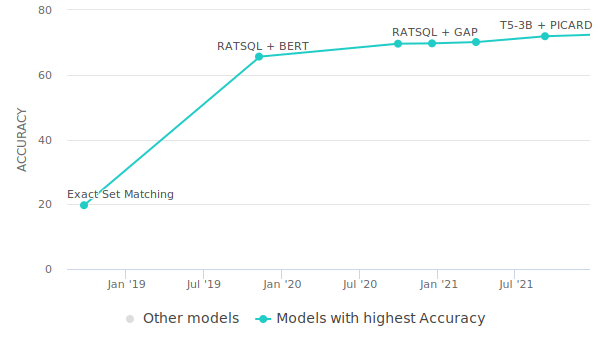
\includegraphics[page=1,width=0.7\textwidth]{pics/picard/benchmark.pdf}
%     \caption{Benchmark results for the PICARD model\cite{picard2020picard}}
% \end{figure}

After the release of Google T5, researchers have been using it to improve the accuracy of text-to-SQL models instead of BERT. New solutions have been released, such as the PICARD with T5-3B model, that significantly improved the SPIDER challenge's accuracy and are motivating researchers to use T5 in their work with innovative approaches since 2021.

\subsubsection{T5}

In Transfer Learning, we start by training our model in an unsupervised fashion on unlabeled data. Then fine-tuning it on a labeled dataset some tasks that we care about, which we call the downstream tasks. For instance, in our unsupervised free training task, we take some text, drop out some of the words, and train the model to predict the missing words. Next, we will fine-tune it on a supervised task like sentiment analysis classifying movie reviews as a given label. This way of training has become an incredible recipe for natural language processing.

T5 Model implemented by Raffel et al. (2020)\cite{raffel_exploring_2020} uses the BERT encoder-decoder architecture proposed by Vaswani et al. (2017) \cite{devlin-etal-2019-bert} and they showed in their studies that it will outperform decoder-only language models. Originally T5 was introduced with five pre-trained models — Small (60 million parameters), Base(220 million parameters), Large(770 million parameters), 3B(3 billion parameters), and 11B(11 billion parameters)\cite{raffel_exploring_2020}.

\begin{figure}[h]
    \centering
    \includegraphics[width=0.5\textwidth]{pics/picard/t5-size.png}
    \caption{T5 models with their Nr. of parameters, layer and feed-forward parameters\cite{raffel_exploring_2020}}
\end{figure}

To pre-train the T5 model, we start with clean text and drop some words to corrupt the text. Each dropped-out span will be replaced with a unique sentinel token, so if multiple words in a row get dropped out, they will be replaced with a single token. The words are dropped out independently uniformly at random so for an inviting get replaced by a single Sentinel token. Then the model is trained to output Sentinel tokens to delineate the dropped-out text corresponding to the text that was dropped out in the input and then each span of dropped-out text.

This method is pretty similar to the span BERT objective. It tried to come up with an objective that was not too different from standard practice.

\begin{figure}[h]
    \centering
    \includegraphics[width=0.6\textwidth]{pics/picard/t5-fine.png}
    \caption{Pre-training by Replace Corrupted Spans \cite{raffel_exploring_2020}}
\end{figure}

Google T5's basic idea is that it models every NLP problem and every text problem as a text-to-text task that takes the text as input and produces text as output.

So fundamentally, it is in a sequence-to-sequence framework; hence, T5 is perfectly suitable for transfer learning machine translation.
T5 can handle various tasks, and it can be fine-tuned for different NLP tasks, such as summarization, COLA (Corpus on linguistic acceptability), classification, multiple text translation, also regression problems like STSB  that predict how similar two sentences are. And in our case Text-to-SQL.

\begin{figure}[h]
    \centering
    \includegraphics[width=0.9\textwidth]{pics/picard/t5-task.png}
    \caption{Each task uses text as input in the model and generates target text. In this way, the same model, loss function, and hyper-parameters are used across various diverse tasks, including translation. \cite{raffel_exploring_2020}}
\end{figure}

Further, because the same model is used for many tasks, the model understands which tasks to perform by prepending a prefix that will also be text.
Therefore, By the end of fine-tuning, T5 will have "n" different models where "n" is the number of tasks. It starts with the same base pre-trained model, and then it is fine-tuned on task A, and then separately, on task B and task C. In our work, we are essentially adding another task to the T5 to handle SQL translation.

\subsubsection*{C4 (Colossal Clean Crawled Corpus)}

The T5 model is pre-trained on C4 Dataset\cite{raffel_exploring_2020}, so its results are quite realistic.
The C4 is an unlabeled dataset gathered and filtered from Common Crawl Dataset, a non-commercial crawler that saves snapshots of the web every month. And web content is dumped out on the order of 20 terabytes.

The cleaning process included deduplication, discarding incomplete sentences, and removing offensive or noisy content. The filtering led to more reliable results on downstream tasks, and the added size let the model size grow without over-fitting when pre-training. C4 is about 750 gigabytes of clean-ish data and is accessible in Tensorflow Datasets Library.


\subsubsection*{Beam Search}
Before understanding the PICARD, let us first understand the concept of Beam Search:

\begin{figure}[h]
    \centering
    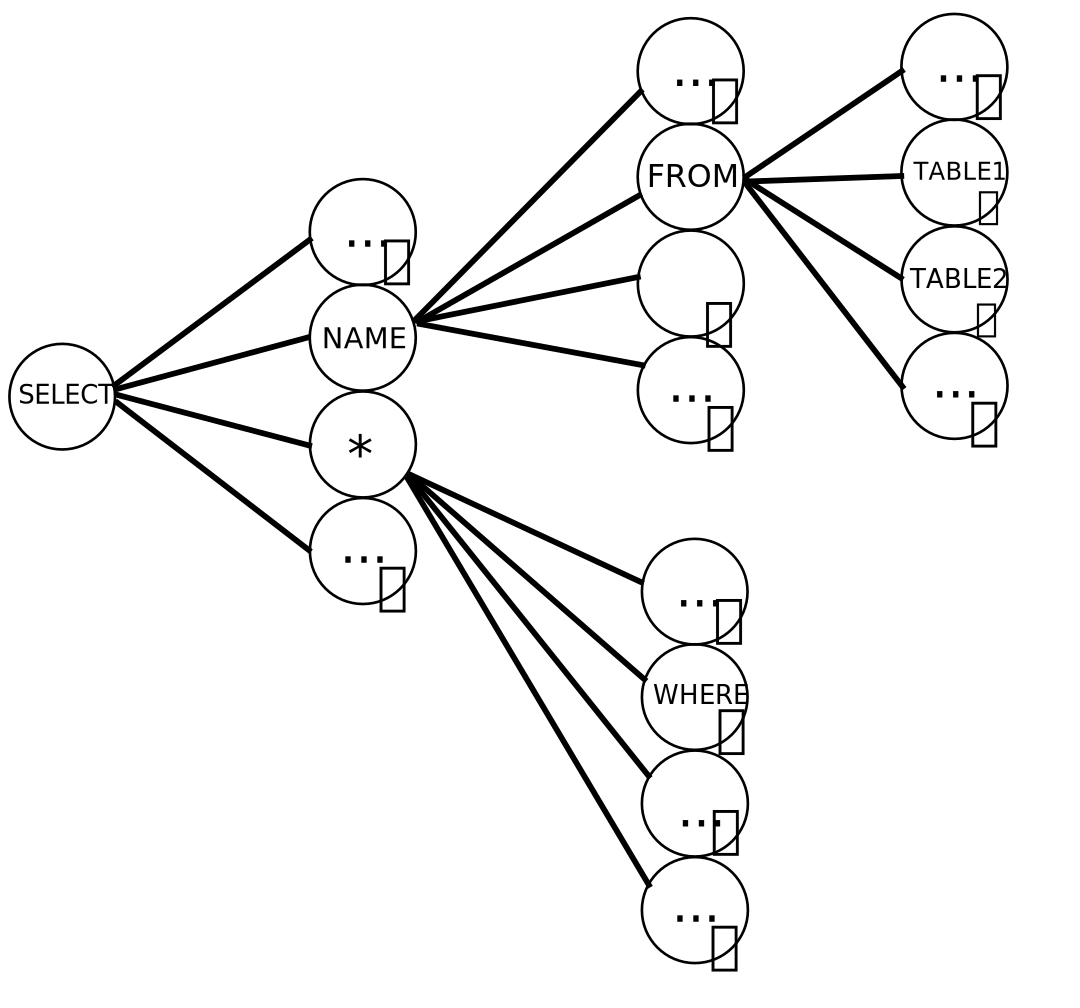
\includegraphics[width=0.6\textwidth]{pics/picard/beam.png}
    \caption{4-Beam Search}
    \label{fig:beam_search}
\end{figure}

Beam search is a widely used search algorithm in natural language processing and machine learning. It is beneficial in sequence-to-sequence (seq2seq) models, which generate output sequences based on input sequences. Beam search is used to find the most likely sequence of output words given an input sequence.
\\
The basic idea behind beam search is to maintain a set of the most likely sequences at each step of the decoding process. This set of sequences, called the "beam," is initially set to the starting point of the decoding process, and at each step, new sequences are generated by considering all the following possible words. The new sequences are then ranked based on their likelihood, and the highest-ranking sequences are added to the beam. The process is repeated until a stopping criterion is met \cite{10.1371/journal.pone.0211558}.
Beam search is handy in seq2seq models because it allows the model to generate multiple output sequences rather than just a single sequence. This is important because, in many cases, there may be multiple valid outputs for a given input sequence. By generating multiple outputs, beam search allows the model to explore the space of possible outputs and find the most likely sequences.
\\
One of the critical advantages of beam search is that it is computationally efficient. Because it only considers a small number of sequences at each step, it can quickly find the most likely sequences without exploring the entire space of possible outputs. This makes it well-suited for use in applications with limited computational resources, such as on mobile devices or in real-time systems.
Another advantage of beam search is that it can be used with other techniques, such as attention mechanisms, to improve the performance of seq2seq models. Attention mechanisms allow the model to focus on specific parts of the input sequence when generating the output, which can help to improve the quality of the generated sequences.
\\
In conclusion, Beam Search is a robust algorithm widely used in natural language processing and machine learning, particularly in the context of sequence-to-sequence (seq2seq) models. It allows the model to generate multiple output sequences rather than just a single sequence and is computationally efficient, making it well-suited for use in applications where computational resources are limited. Additionally, it can be combined with other techniques, such as attention mechanisms, to improve the performance of seq2seq models.

\subsubsection{PICARD}

% PICARD\cite{Scholak2021:PICARD} stands for "Parsing Incrementally for Constrained Auto-Regressive Decoding.". It can be used with any existing language model decoder or vocabulary based on auto-regressive language modeling.

% PICARD allows for the generation of executable code by constraining the output of the language model to be syntactically and semantically correct. It does this by integrating with standard beam search, a technique used in natural language processing to generate a sequence of words or tokens by expanding a beam of hypotheses step by step. At each decoding step, PICARD checks whether the most likely tokens are valid and if not, it discards them. PICARD is compatible with any model that generates a sequence of tokens and can be used with character, subword, and word-level language models without requiring exceptional recovery.

PICARD\cite{Scholak2021:PICARD}, short for "Parsing Incrementally for Constrained Auto-Regressive Decoding," is a method that can be used in conjunction with any language model decoder or vocabulary that utilizes auto-regressive language modeling.

PICARD is a technique that utilizes standard beam search, commonly used in natural language processing, to generate executable code by ensuring the output of the language model is both syntactically and semantically correct. It works by expanding a beam of hypotheses step by step and discarding any tokens that are not valid at each decoding step. This method can be applied to any language model that generates a sequence of tokens, including character, subword, and word-level models, without requiring unique recovery methods.

It effectively improves the performance of existing models and achieves state-of-the-art performance on tasks such as text-to-SQL translation.
Warps model prediction scores and integrates trivially with existing greedy and beam search algorithms used in auto-regressive decoding from language models.

At each generation step, Picard first restricts prediction to the top-k highest probability tokens and then assigns a score of negative infinity to those that fail Picard's numerous checks.

PICARD has four modes that control the level of comprehensiveness of its checking process: off, lexing, parsing without guards, and parsing with guards, with the latter being the most comprehensive. In lexing mode, PICARD checks if the current token is a valid keyword or identifier. In parsing guard mode, it checks if the current token is a valid keyword or identifier, a valid SQL keyword, and a valid SQL identifier.

Picard can detect spelling errors in keywords or reject table and column names that are invalid for the given SQL schema.
"Out-of-distribution compositional generalization and natural language variation" refers to the ability of a natural language processing (NLP) system to handle novel combinations of words and phrases that it has not seen before while also being able to handle variations in language usage.
Compositional generalization refers to the ability of an NLP system to understand and generate novel combinations of words and phrases by using its knowledge of the meanings and relationships of individual words and phrases. This is an essential aspect of NLP because it allows the system to understand and generate language flexibly and adaptively.

The concept of natural language variation refers to the multiple ways people can express the same ideas or concepts using natural language. This can include variations in dialect, style, or tone, which can make it difficult for NLP systems to understand and generate language accurately.

Together, out-of-distribution compositional generalization and natural language variation represent fundamental challenges in the field of NLP. They require NLP systems to handle a wide range of language input and output in order to be effective.

PICARD can be applied as an optional feature during inference but is not necessarily included in pre-training or fine-tuning, and for text-to-SQL translation, it works directly on the output of the language model. PICARD has been shown to have state-of-the-art performance on complex Spider text-to-SQL translation tasks, achieving an accuracy of 75.1\%.

Picard warps model prediction scores and integrates trivially with existing greedy and beam search algorithms. In addition to the token ids of the current hypothesis, the model's language modeling head also predicts the log-softmax scores for each vocabulary token. Additionally, Picard has access to SQL schema information, including table and column names and which column resides in which table.

Motivated by the success of Shaw et al. \cite{shaw-etal-2021-compositional}, who demonstrated that a pre-trained T5-Base or T5-3B model could effectively learn the text-to-SQL task, generalize to never-before-seen databases, and even rival the state-of-the-art methods of Choi et al.\cite{10.1162/coli_a_00403} without any modifications to the model itself, the researchers opted to use T5 as the baseline for all their experiments. The results from Shaw et al.\cite{shaw-etal-2021-compositional} suggest that T5-based models had the potential to improve the field of natural language processing significantly. Therefore, the researchers sought to take advantage of the capabilities of T5 in order to gain new insights into how natural language can be effectively utilized to solve complex tasks.
\subsubsection{Beam Search}
Before understanding the PICARD, let us first understand the concept of Beam Search:

\begin{figure}[H]
    \centering
    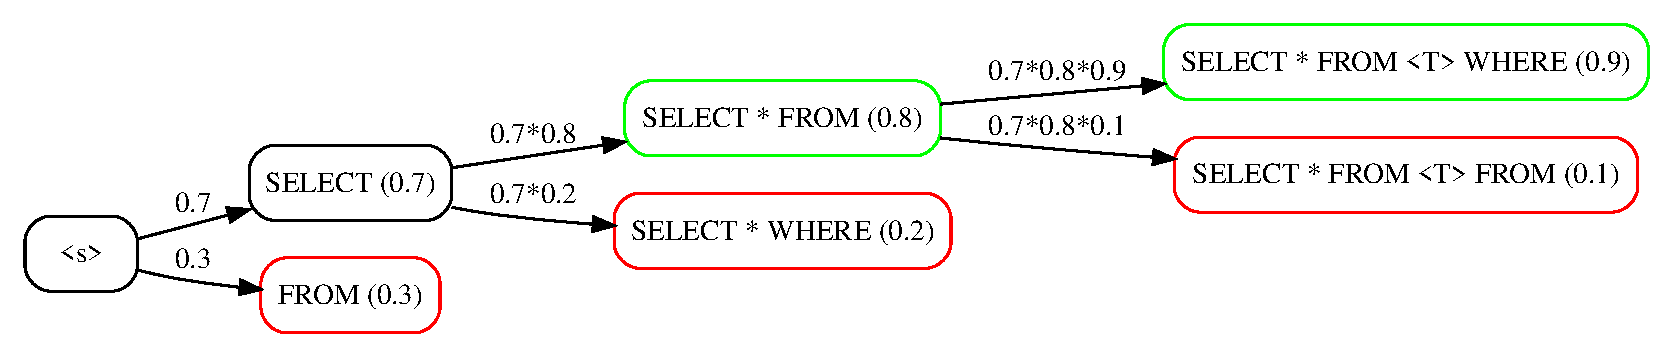
\includegraphics[width=0.8\textwidth]{pics/picard/beam/beam.eps}
    \caption{2-Beam Search}
    \label{fig:beam_search}
\end{figure}

Beam search is a widely used search algorithm in natural language processing and machine learning. It is beneficial in sequence-to-sequence (seq2seq) models, which generate output sequences based on input sequences. Beam search is used to find the most likely sequence of output words given an input sequence.
\\
The basic idea behind beam search is to maintain a set of the most likely sequences at each step of the decoding process. This set of sequences called the "beam," is initially set to the starting point of the decoding process, and at each step, new sequences are generated by considering all the following possible words. The new sequences are then ranked based on their likelihood, and the highest-ranking sequences are added to the beam. The process is repeated until a stopping criterion is met \cite{10.1371/journal.pone.0211558}.
Beam search is handy in seq2seq models because it allows the model to generate multiple output sequences rather than just a single sequence. This is important because, in many cases, there may be multiple valid outputs for a given input sequence. By generating multiple outputs, beam search allows the model to explore the space of possible outputs and find the most likely sequences.
\\
One of the critical advantages of beam search is that it is computationally efficient. Because it only considers a small number of sequences at each step, it can quickly find the most likely sequences without exploring the entire space of possible outputs. This makes it well-suited for use in applications with limited computational resources, such as on mobile devices or in real-time systems.
Another advantage of beam search is that it can be used with other techniques, such as attention mechanisms, to improve the performance of seq2seq models. Attention mechanisms allow the model to focus on specific parts of the input sequence when generating the output, which can help to improve the quality of the generated sequences.
\\
In conclusion, Beam Search is a robust algorithm widely used in natural language processing and machine learning, particularly in the context of sequence-to-sequence (seq2seq) models. It allows the model to generate multiple output sequences rather than just a single sequence and is computationally efficient, making it well-suited for use in applications where computational resources are limited. Additionally, it can be combined with other techniques, such as attention mechanisms, to improve the performance of seq2seq models.
\clearpage

\subsection{T5 + PICARD} \label{picard}

% \begin{figure}[h]
%     \centering
%     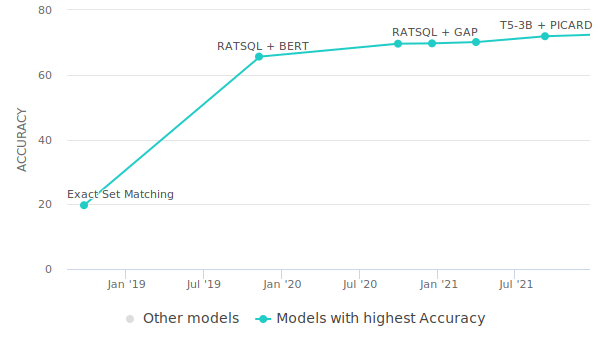
\includegraphics[page=1,width=0.7\textwidth]{pics/picard/benchmark.pdf}
%     \caption{Benchmark results for the PICARD model\cite{picard2020picard}}
% \end{figure}

After the release of Google T5, researchers have been using it to improve the accuracy of text-to-SQL models instead of BERT. New solutions have been released, such as the PICARD with T5-3B model, that significantly improved the SPIDER challenge's accuracy and are motivating researchers to use T5 in their work with innovative approaches since 2021.

\subsubsection{T5}

In Transfer Learning, we start by training our model in an unsupervised fashion on unlabeled data. Then fine-tuning it on a labeled dataset some tasks that we care about, which we call the downstream tasks. For instance, in our unsupervised free training task, we take some text, drop out some of the words, and train the model to predict the missing words. Next, we will fine-tune it on a supervised task like sentiment analysis classifying movie reviews as a given label. This way of training has become an incredible recipe for natural language processing.

T5 Model implemented by Raffel et al. (2020)\cite{raffel_exploring_2020} uses the BERT encoder-decoder architecture proposed by Vaswani et al. (2017) \cite{devlin-etal-2019-bert} and they showed in their studies that it will outperform decoder-only language models. Originally T5 was introduced with five pre-trained models — Small (60 million parameters), Base(220 million parameters), Large(770 million parameters), 3B(3 billion parameters), and 11B(11 billion parameters)\cite{raffel_exploring_2020}.

\begin{figure}[h]
    \centering
    \includegraphics[width=0.5\textwidth]{pics/picard/t5-size.png}
    \caption{T5 models with their Nr. of parameters, layer and feed-forward parameters\cite{raffel_exploring_2020}}
\end{figure}

To pre-train the T5 model, we start with clean text and drop some words to corrupt the text. Each dropped-out span will be replaced with a unique sentinel token, so if multiple words in a row get dropped out, they will be replaced with a single token. The words are dropped out independently uniformly at random so for an inviting get replaced by a single Sentinel token. Then the model is trained to output Sentinel tokens to delineate the dropped-out text corresponding to the text that was dropped out in the input and then each span of dropped-out text.

This method is pretty similar to the span BERT objective. It tried to come up with an objective that was not too different from standard practice.

\begin{figure}[h]
    \centering
    \includegraphics[width=0.6\textwidth]{pics/picard/t5-fine.png}
    \caption{Pre-training by Replace Corrupted Spans \cite{raffel_exploring_2020}}
\end{figure}

Google T5's basic idea is that it models every NLP problem and every text problem as a text-to-text task that takes the text as input and produces text as output.

So fundamentally, it is in a sequence-to-sequence framework; hence, T5 is perfectly suitable for transfer learning machine translation.
T5 can handle various tasks, and it can be fine-tuned for different NLP tasks, such as summarization, COLA (Corpus on linguistic acceptability), classification, multiple text translation, also regression problems like STSB  that predict how similar two sentences are. And in our case Text-to-SQL.

\begin{figure}[h]
    \centering
    \includegraphics[width=0.9\textwidth]{pics/picard/t5-task.png}
    \caption{Each task uses text as input in the model and generates target text. In this way, the same model, loss function, and hyper-parameters are used across various diverse tasks, including translation. \cite{raffel_exploring_2020}}
\end{figure}

Further, because the same model is used for many tasks, the model understands which tasks to perform by prepending a prefix that will also be text.
Therefore, By the end of fine-tuning, T5 will have "n" different models where "n" is the number of tasks. It starts with the same base pre-trained model, and then it is fine-tuned on task A, and then separately, on task B and task C. In our work, we are essentially adding another task to the T5 to handle SQL translation.

\subsubsection*{C4 (Colossal Clean Crawled Corpus)}

The T5 model is pre-trained on C4 Dataset\cite{raffel_exploring_2020}, so its results are quite realistic.
The C4 is an unlabeled dataset gathered and filtered from Common Crawl Dataset, a non-commercial crawler that saves snapshots of the web every month. And web content is dumped out on the order of 20 terabytes.

The cleaning process included deduplication, discarding incomplete sentences, and removing offensive or noisy content. The filtering led to more reliable results on downstream tasks, and the added size let the model size grow without over-fitting when pre-training. C4 is about 750 gigabytes of clean-ish data and is accessible in Tensorflow Datasets Library.


\subsubsection*{Beam Search}
Before understanding the PICARD, let us first understand the concept of Beam Search:

\begin{figure}[h]
    \centering
    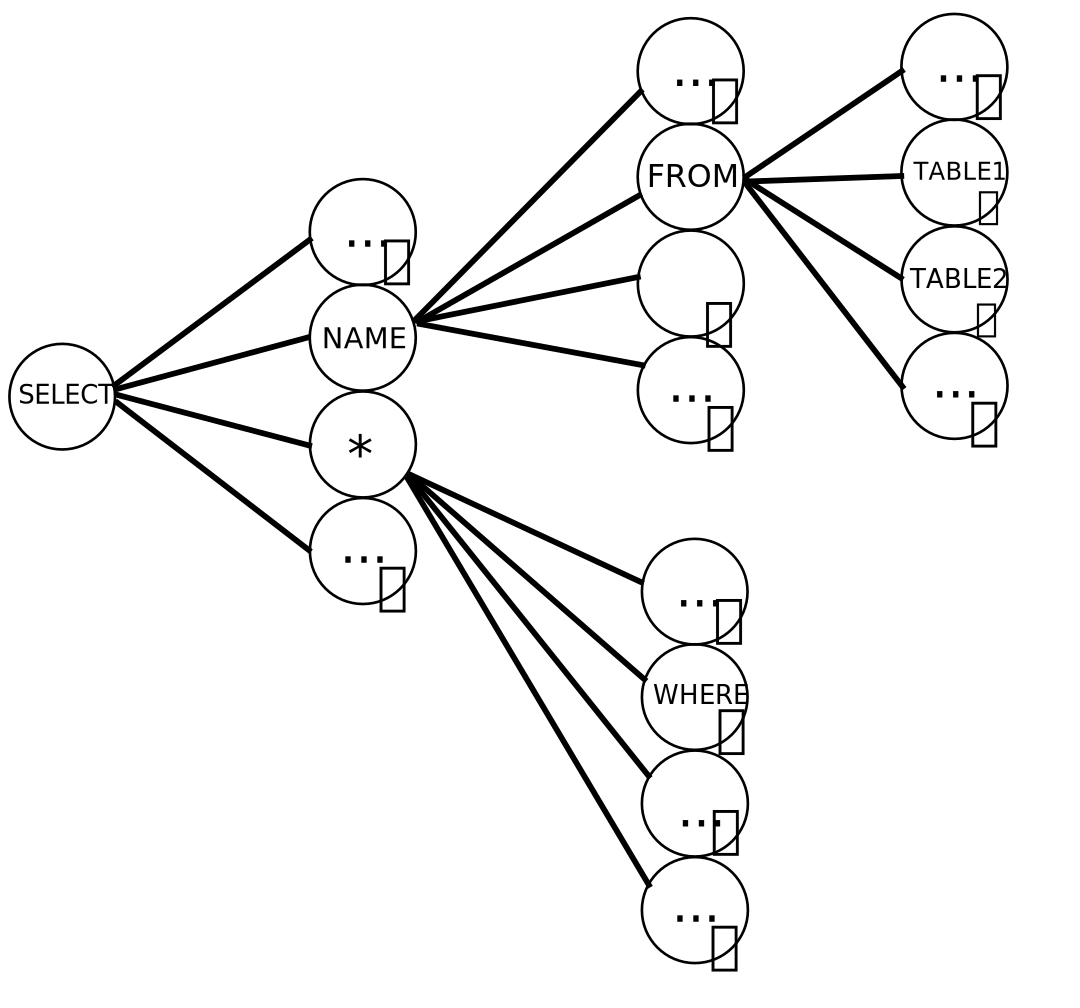
\includegraphics[width=0.6\textwidth]{pics/picard/beam.png}
    \caption{4-Beam Search}
    \label{fig:beam_search}
\end{figure}

Beam search is a widely used search algorithm in natural language processing and machine learning. It is beneficial in sequence-to-sequence (seq2seq) models, which generate output sequences based on input sequences. Beam search is used to find the most likely sequence of output words given an input sequence.
\\
The basic idea behind beam search is to maintain a set of the most likely sequences at each step of the decoding process. This set of sequences, called the "beam," is initially set to the starting point of the decoding process, and at each step, new sequences are generated by considering all the following possible words. The new sequences are then ranked based on their likelihood, and the highest-ranking sequences are added to the beam. The process is repeated until a stopping criterion is met \cite{10.1371/journal.pone.0211558}.
Beam search is handy in seq2seq models because it allows the model to generate multiple output sequences rather than just a single sequence. This is important because, in many cases, there may be multiple valid outputs for a given input sequence. By generating multiple outputs, beam search allows the model to explore the space of possible outputs and find the most likely sequences.
\\
One of the critical advantages of beam search is that it is computationally efficient. Because it only considers a small number of sequences at each step, it can quickly find the most likely sequences without exploring the entire space of possible outputs. This makes it well-suited for use in applications with limited computational resources, such as on mobile devices or in real-time systems.
Another advantage of beam search is that it can be used with other techniques, such as attention mechanisms, to improve the performance of seq2seq models. Attention mechanisms allow the model to focus on specific parts of the input sequence when generating the output, which can help to improve the quality of the generated sequences.
\\
In conclusion, Beam Search is a robust algorithm widely used in natural language processing and machine learning, particularly in the context of sequence-to-sequence (seq2seq) models. It allows the model to generate multiple output sequences rather than just a single sequence and is computationally efficient, making it well-suited for use in applications where computational resources are limited. Additionally, it can be combined with other techniques, such as attention mechanisms, to improve the performance of seq2seq models.

\subsubsection{PICARD}

% PICARD\cite{Scholak2021:PICARD} stands for "Parsing Incrementally for Constrained Auto-Regressive Decoding.". It can be used with any existing language model decoder or vocabulary based on auto-regressive language modeling.

% PICARD allows for the generation of executable code by constraining the output of the language model to be syntactically and semantically correct. It does this by integrating with standard beam search, a technique used in natural language processing to generate a sequence of words or tokens by expanding a beam of hypotheses step by step. At each decoding step, PICARD checks whether the most likely tokens are valid and if not, it discards them. PICARD is compatible with any model that generates a sequence of tokens and can be used with character, subword, and word-level language models without requiring exceptional recovery.

PICARD\cite{Scholak2021:PICARD}, short for "Parsing Incrementally for Constrained Auto-Regressive Decoding," is a method that can be used in conjunction with any language model decoder or vocabulary that utilizes auto-regressive language modeling.

PICARD is a technique that utilizes standard beam search, commonly used in natural language processing, to generate executable code by ensuring the output of the language model is both syntactically and semantically correct. It works by expanding a beam of hypotheses step by step and discarding any tokens that are not valid at each decoding step. This method can be applied to any language model that generates a sequence of tokens, including character, subword, and word-level models, without requiring unique recovery methods.

It effectively improves the performance of existing models and achieves state-of-the-art performance on tasks such as text-to-SQL translation.
Warps model prediction scores and integrates trivially with existing greedy and beam search algorithms used in auto-regressive decoding from language models.

At each generation step, Picard first restricts prediction to the top-k highest probability tokens and then assigns a score of negative infinity to those that fail Picard's numerous checks.

PICARD has four modes that control the level of comprehensiveness of its checking process: off, lexing, parsing without guards, and parsing with guards, with the latter being the most comprehensive. In lexing mode, PICARD checks if the current token is a valid keyword or identifier. In parsing guard mode, it checks if the current token is a valid keyword or identifier, a valid SQL keyword, and a valid SQL identifier.

Picard can detect spelling errors in keywords or reject table and column names that are invalid for the given SQL schema.
"Out-of-distribution compositional generalization and natural language variation" refers to the ability of a natural language processing (NLP) system to handle novel combinations of words and phrases that it has not seen before while also being able to handle variations in language usage.
Compositional generalization refers to the ability of an NLP system to understand and generate novel combinations of words and phrases by using its knowledge of the meanings and relationships of individual words and phrases. This is an essential aspect of NLP because it allows the system to understand and generate language flexibly and adaptively.

The concept of natural language variation refers to the multiple ways people can express the same ideas or concepts using natural language. This can include variations in dialect, style, or tone, which can make it difficult for NLP systems to understand and generate language accurately.

Together, out-of-distribution compositional generalization and natural language variation represent fundamental challenges in the field of NLP. They require NLP systems to handle a wide range of language input and output in order to be effective.

PICARD can be applied as an optional feature during inference but is not necessarily included in pre-training or fine-tuning, and for text-to-SQL translation, it works directly on the output of the language model. PICARD has been shown to have state-of-the-art performance on complex Spider text-to-SQL translation tasks, achieving an accuracy of 75.1\%.

Picard warps model prediction scores and integrates trivially with existing greedy and beam search algorithms. In addition to the token ids of the current hypothesis, the model's language modeling head also predicts the log-softmax scores for each vocabulary token. Additionally, Picard has access to SQL schema information, including table and column names and which column resides in which table.

Motivated by the success of Shaw et al. \cite{shaw-etal-2021-compositional}, who demonstrated that a pre-trained T5-Base or T5-3B model could effectively learn the text-to-SQL task, generalize to never-before-seen databases, and even rival the state-of-the-art methods of Choi et al.\cite{10.1162/coli_a_00403} without any modifications to the model itself, the researchers opted to use T5 as the baseline for all their experiments. The results from Shaw et al.\cite{shaw-etal-2021-compositional} suggest that T5-based models had the potential to improve the field of natural language processing significantly. Therefore, the researchers sought to take advantage of the capabilities of T5 in order to gain new insights into how natural language can be effectively utilized to solve complex tasks.

% Schema linking is a component of text-to-SQL models that helps map natural language phrases to elements of a database schema.
% Skeleton parsing is a component of text-to-SQL models that helps generate the structure of an SQL query based on a natural language question. It focuses on generating the pure skeleton of an SQL query (i.e., SQL keywords).